\chapter{Context}
\begin{figure}
\centering
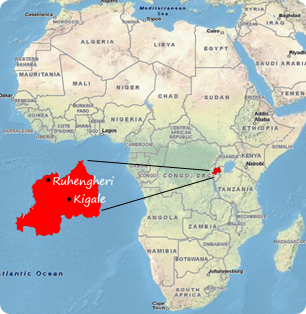
\includegraphics[width=12cm]{empirical/images/context_map_rwanda}
\label{context_map_of_rwanda}
\caption{Rwanda in the World \cite{14}}
\end{figure}
In the center of Africa we find Rwanda. A very small country, only \(26338 km^2\). This would be about 7\% of Norway. 
Their population is estimated to be around 12 million wich makes it about 420 people pr. square kilometer. 
Rwanda is made up of 5 provinces, east, west, north, south and Kigali. 
Each province is again divided into districts and there is a total of 30 districts. Under districts there is a total of 416 sectors\cite{1}.
\begin{figure}
\centering
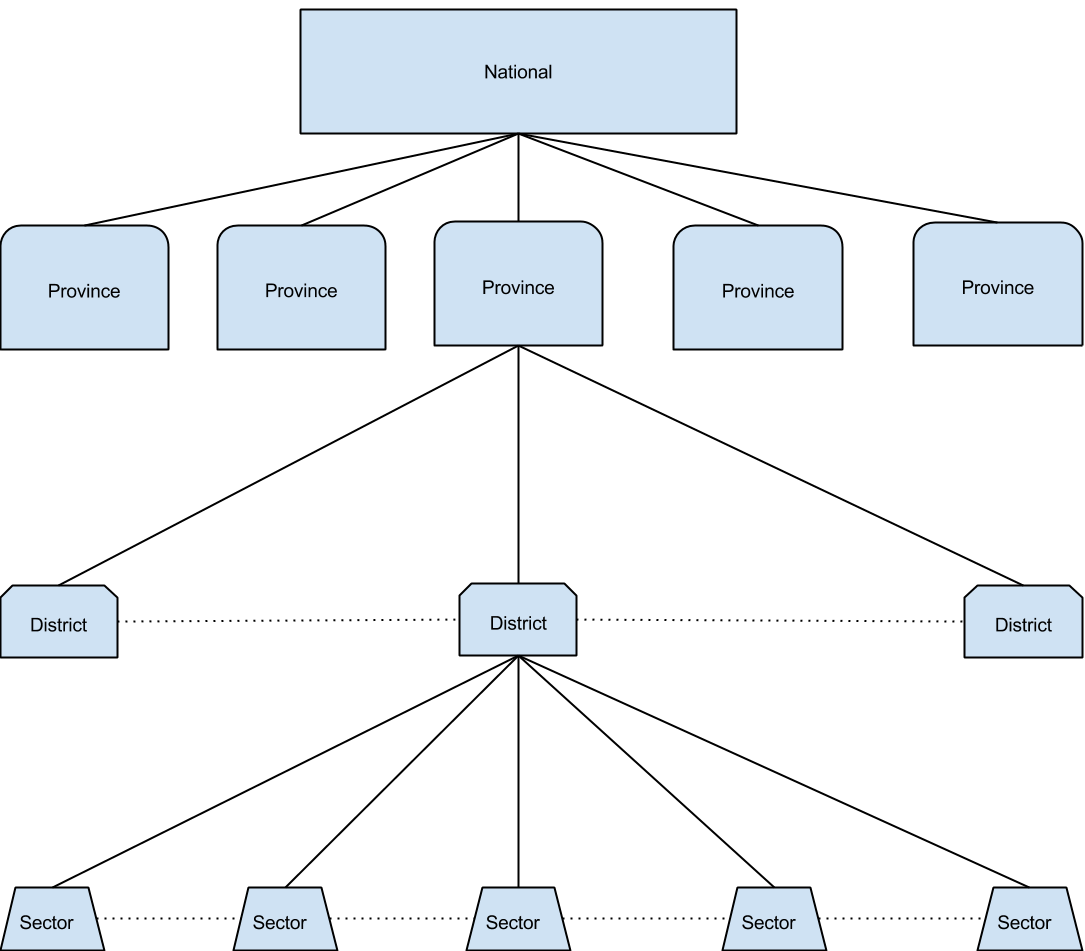
\includegraphics[width=12cm]{empirical/images/rwanda_administrative_division}
\caption{Rwanda Administrative Division}
\end{figure}
Because of its location it works perfect as a gateway to all countries in Africa. 
And due to the stable environment compared to many other contries in this part of the world, it is very attractive for foreigners to do business here. 
Making it the `Singapore of Africa'.

Rwanda has a goal of being transformed to a knowledge based economy with Information and Communication Technology or ICT. 
This means basicly that they want to offer ICT services for other kind of resources. 
They want to be the regional center for training top quality ICT\nomenclature{ICT}{Information and Communication Technology} professionals.
In turn, create wealth, jobs and entreprenaurs. 
From their perspective they have some competetive advantages in order to achieve this:
\begin{itemize}
\item Cheap labor compared to other countries in the Region
\item Young and dynamic workforce (98\% of the population is under 50 years and 43\% is under 16 years)
\item Most favorable business environment in the Region (8th best place to do business in the world 2012)
\item Low levels of corruption - Zero tolerance (Transparency international Bribery index 2012 ranked Rwanda as least bribery prone in the EAC)
\item World class ICT infrastructure
\item Strong \& visionary leadership
\item Bi-lingual business environment (French and English)
\end{itemize}
\cite{2}

\section{Brief History Lesson}
We start at the 14th centuary, when the Tutsies enters Rwanda. 
Before them there were two other peoples, Hutu, which means farmers and Twa who was the very first recorded prople in Rwanda.
There is some disagreement of what the differances are between the peoples, but origanily, Tutsies were cattle owners and the Hutus were farmers. 
About five hundred years later the first European visits Rwanda and in the same centuary Rwanda becomes a german protectorate. 
This makes Rwanda under the protection of Germany with some oblegations for their services.
Skipping fourth to 1933, now occupied by Belgian forces, all citizens are issued with an identity card defining their identity.
In 1962 Rwanda becomes independent and gets their 1st elected President. 
After this there is turbulent times for Rwanda. The Hutus and Tutsies are having violent reactions towards eachother with a peak in 1994.
A geneside primeraly by Hutu extremists, killed over 500,000 people, primeraly Tutsies, in the course of about 100 days. 
The genocide was triggered by the assasination of the Hutu president Habyarimana.  
The Tutsie Rwandian Patriotic Front, also known as the RPF\nomenclature{RPF}{Rwandian Patriotic Front}, takes action and took control of Rwanda the same year.
The current President, Paul Kagame, was a former member of the Rwandian Patriotic Front.
\cite{17}\cite{18}\cite{19}

\section{Information Technology focus in Rwanda}

\begin{figure}
\centering
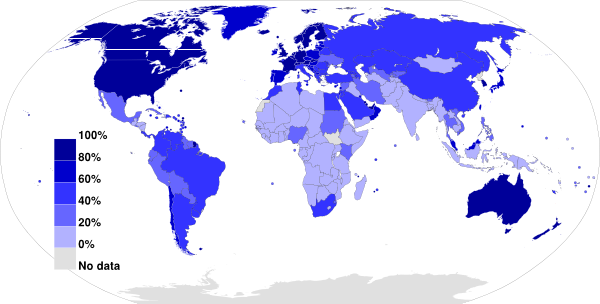
\includegraphics[width=12cm]{empirical/images/internet_penetration_2012}
\caption{Global Internet Penetration in 2012 \cite{3}}
\label{fig:global_internet_penetration_2012}
\end{figure}

\begin{figure}
\centering
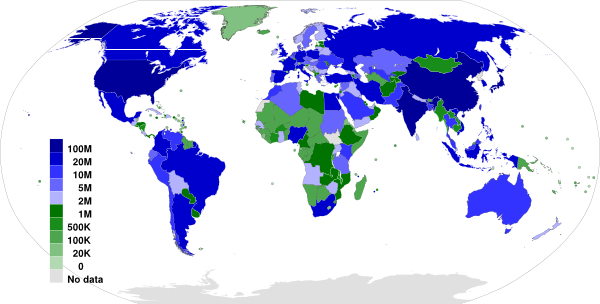
\includegraphics[width=12cm]{empirical/images/internet_users_2012}
\caption{Global Internet Users in 2012 \cite{3}}
\label{fig:global_internet_users_2012}
\end{figure}

Rwanda has an internet penetration of 7\% in 2012. 
In Africa there is an internet penetration of 15.6\% and for the world it is 34.3\% (See ~\ref{fig:global_internet_penetration_2012})\cite{4}. 
Rwanda had an increase of internet penetration from 1\% to 7\% from 2000 to the end of 2011\cite{2}.
More interesting is the mobile broadband development in Rwanda. 
The subscriber base accounts for 48.1\% of the population and the network coverage accounts for 99.79\% of the country.
Thus, the technology is there, but the hardware is not yet updated.
In general, people are using simple phones.
Some of these phones supports java and a very simple browser, but it cannot be compared to a working internet connection.
The government of Rwanda has made the decision to become an ICT hub in Africa.
Therefore alot of resources and attention is focused on developing knowledge in the field of ICT. 
As of january 2013 the Rwandian government is planning to set up an ICT park through the Rwanda Development Board.
This park will host technological training, industries research and development. The ICT park will support the growth of the following clusters:
\begin{itemize}
\item Energy
\item Internet, multimedia and mobile telecommunication
\item Knowledge
\item E-Government
\item Financial
\item ICT Service and export
\end{itemize}
\cite{2}
Also there were some rumors about free WiFi throughout all of Kigali.
They were in 2012 ranked among the top 6 developing countries when it comes to dynamic performance in ICT development\cite{5}.

\section{Health Information System Programme}
\subsection{About}
The Health Information Systems Programme (HISP) is a global network established, managed and coordinated by the Department of Informatics at the University of Oslo.
They design, implement and sustain Health Information Systems by a participatory approach\cite{8}. 
This means including the local users when develping the system in hopes of a more sustainable and successful project.
The system developed aims for supporting health care delivery and informaiton flows in selected health facilities, districts and provinces.
\begin{description}
\item[Vision] To strengthen the development and use of integrated health information systems within a public health inspired framework in India and the South Asian region\cite{9}.
\item[Mission] To enable networks of collaborative action with like-minded actors who aspire to the ideology of open source software, open standards and decentralized decision-making to create complementary strengths in providing integrated and public health friendly health information systems\cite{9}.
\subsection{History}
In the 1970 and 80's the HISP\nomenclature{HISP}{Health Information System Programme} approach to action research and system design was influenced by a number of union based action research projects in Scandinavia.
The focus were on empowering workers who were affected or threatened by new technology.
Methods may have changed over time, but the philosophy remains the same.
Explore ways in wich disadvantaged people could appropriate ICT's for their own empowerment.
Original key member of the HISP team had background as social political activists in the anti-apartheid struggle and other social movements.
DHIS\nomenclature{DHIS}{District Health Information System}, a software organized and developed within the HISP network, was actually born out of the political processes following the fall of apartheid\cite{7}. 
During apartheid and until 1994 there were 14 departments of health in South Africa.
Bacause of this fragmantation it was alot of different procedures, collection tools and data defenitions. 
In order to take this into account, DHIS became very flexible and one can easily see how this has effected the design. 
This might be the reason why DHIS framework could be used in other countries.

\subsection{District Health Information System}
\label{sec:dhis}
The latest version of DHIS during the case study was version 2.13.
DHIS2 is now used by over 30 countries across the globe and even more organizations.
DHIS2 is a tool for governments and health organizations to manage their operations more effectively, monitor processes and improve communication.
DHIS2 is mainly a tool for managing aggregate data. 
It will let you visualize large amounts of data in a GIS\nomenclature{GIS}{Graphical Information System} implementation, a pivot table and in charts. 
These data representations can then be shared with other user registred in the same DHIS2 instance.
Probably the most powerful feature would be GIS. 
This feature shows selected data on map based on province, district etc\nomenclature{etc}{Et cetera}. 
The regions on the map can then be colored based on the data. 
If one has data for the hole country one can in seconds get a accurate impression of the current health status. 
DHIS2 runs on server wich is connected to a database. 
As long as this server is connected, anyone with a decent browser and an internet connection could access and make use of DHIS2.
\subsubsection{GIS}
\begin{figure}
\centering
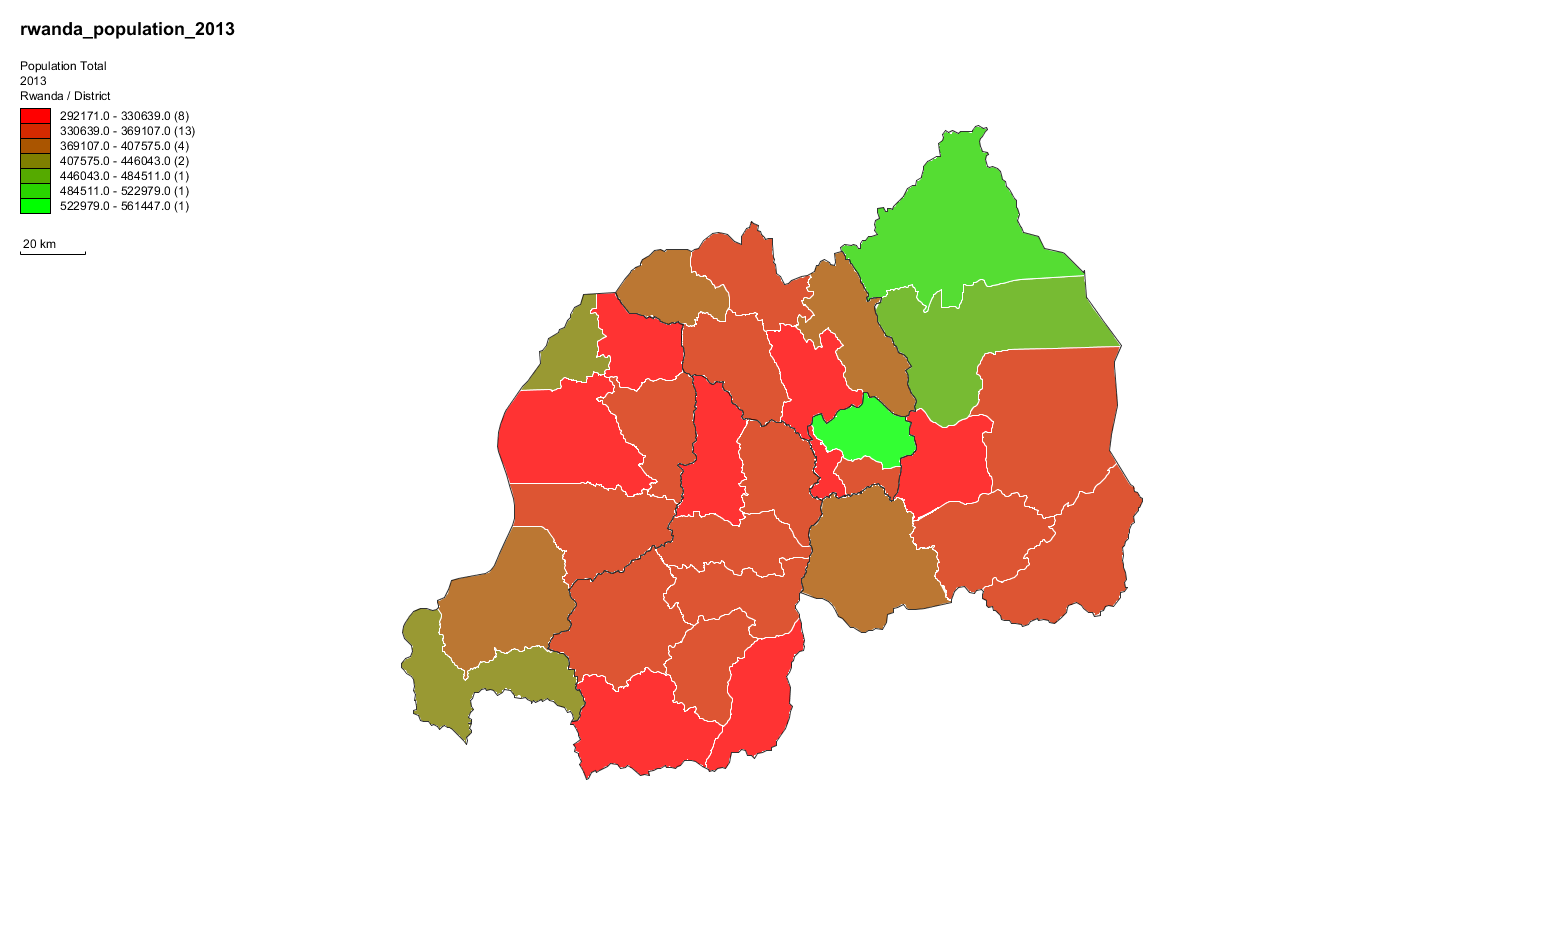
\includegraphics[width=12cm]{empirical/images/map_rwanda_population_2013}
\caption{A population count using GIS in DHIS2}
\label{fig:a_population_count_using_gis_in_dhis2}
\end{figure}
The GIS that is integrated in DHIS2 is relatively easy to use. 
One selects what kind of regions that are of interest and apply the correct data that should be visualized, see figure ~\ref{fig:a_population_count_using_gis_in_dhis2}.
Heres a list of some of the functionality that the GIS offers:
\begin{itemize}
\item Thematic mapping of areas and points.
\item Visualize catchment areas of facilities.
\item View facilites based on classifications.
\item Overlay multiple layers and use googlemaps as a background layer.
\end{itemize}\cite{10}
\subsubsection{Charts}
\begin{figure}
\centering
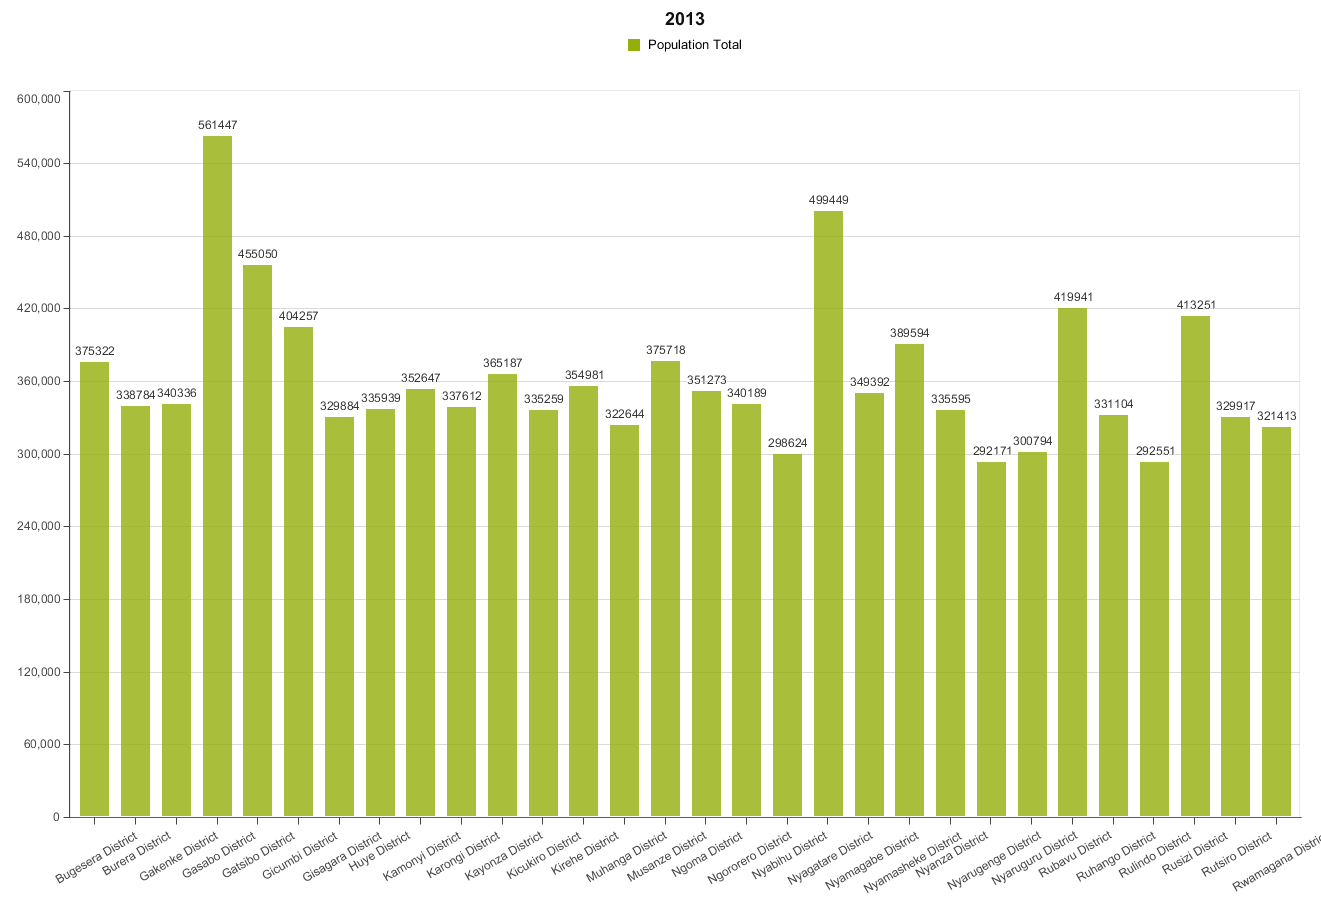
\includegraphics[width=12cm]{empirical/images/chart_rwanda_population_2013}
\caption{A population count using a chart in DHIS2}
\label{fig:a_population_count_using_a_chart_in_dhis2}
\end{figure}
The charts are a little bit trickier. In short the series is the y-axis and Category is the x-axis. Displaying data as a chart is allright once you get what the words mean.
Figure \ref{fig:a_population_count_using_a_chart_in_dhis2} shows an example counting population by district. Types of charts supported include:
\begin{itemize}
\item Column
\item Line
\item Pie
\item Stacked Column
\item Area
\end{itemize}
\cite{10}
\subsubsection{Pivot Table}
\begin{figure}
\centering
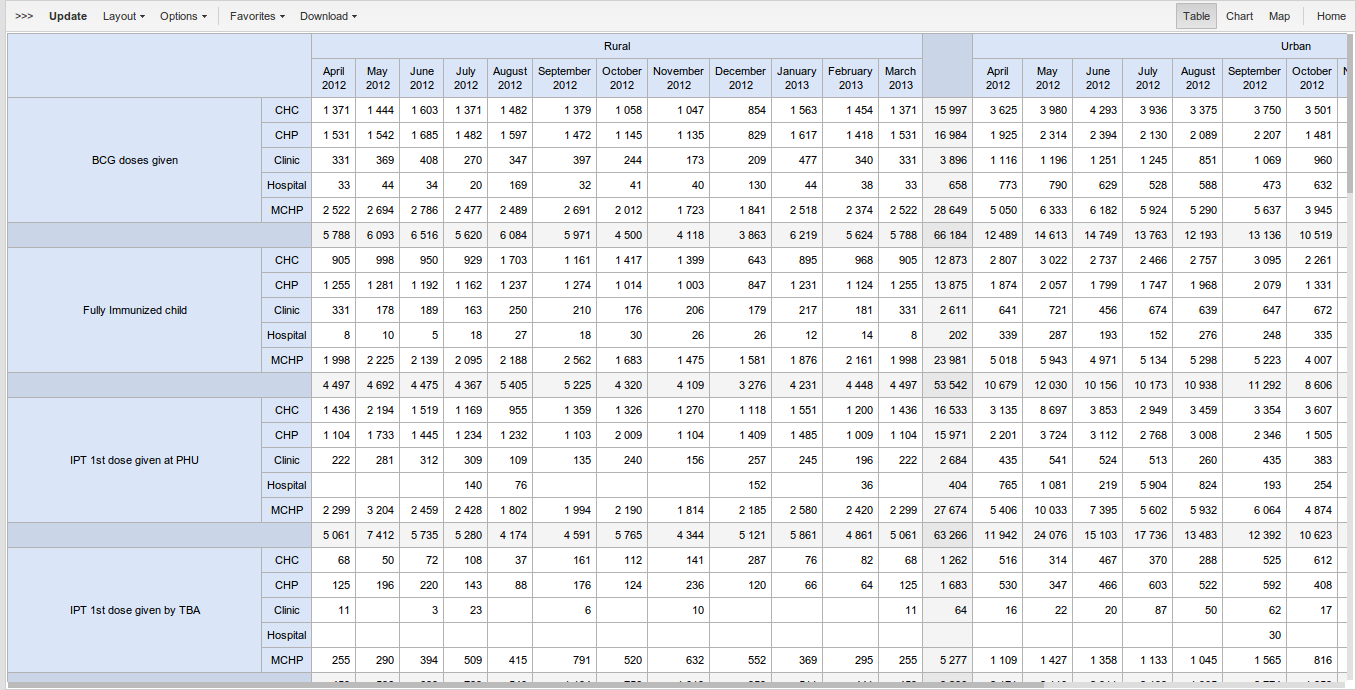
\includegraphics[width=12cm]{empirical/images/pivot_table_example}
\caption{An example of a pivot table in DHIS2\cite{10}}
\label{an_example_of_a_pivot_table_in_dhis2}
\end{figure}
A pivot table is a data summarization tool. It generally sorts data and show them in categorized table.
The DHIS2 pivot table let's you analyse data along all data dimensions and arrange these on columns, rows and filters, see \ref{an_example_of_a_pivot_table_in_dhis2}.
\subsubsection{Dashboard and social features}
One can send messages and share all data visualizations with users registrered on the DHIS2 instance. Interpretations of the visualizations can be commented and viewed by all other users. 
This way DHIS2 let's users experienced in the field help others interpretate the data while they are looking at it. Also one can store charts, maps and pivot table at a dashboard so they can easily be referenced later.
\subsubsection{Individual Records}
DHIS2 was mainly intended for aggregated data that could not related to anyone person. The need for a system which can track individuals is a requirement that most users of a health care system would want.
Therefore the DHIS2 tracker was developed. It let's you sign up people for programs and track them through the process. Also send out reminders so that patients come to their scheduled checkups. 
One problem with the individual records is that it does not work as a patient record system. Such a system is that it requires a level of confidenciality that DHIS2 currently is not supporting. 
Also a patient record system needs all health facillities to be users of the same system if it is going to be of any use.
\subsubsection{Data entry and validation}
DHIS2 let's users entry data even if their not online. 
This feature is crucial for countries with unreliable connection to the internet. 
For developing countries with regular power cuts, one can understand why this is. 
Data entry is done with prepared forms and then uploaded to the server which is running the DHIS2 instance.
The forms are highly customizable due to the varying requirements from users. 
Also there is the possibility to validate the input. For an example shouldn't there be more people under five years than people in the same region, just to give an example.
The data entry can be done in alot of different ways. 
One example is through SMS\nomenclature{SMS}{Simple Message Service}. In industy countries this may sound odd at first, but in developing countries health facilities might not have access to computers. 
This is the simplest form of data entry, even though it might require some coding of data representations. 
Since DHIS2 is accessible from any device with a browser the range of devices that can be used for data entry goes from a mobile phone that supports SMS to a sophisticated computer. 

\section{Healthcare}
The health care in Rwanda is still influenced by the genocide in 94, but compared to the state it was in back then, it's is in pretty good shape.
The health system is financed primarely the state, insurrance, individuals and direct fees for services.
The biggest health program is the Mutuelles De Sante. This is an insurrance based scheme.
Individuals pay a fee of 6\$ a year pr. family member and 10\% fo the service pr. visit.
The program started in 2004 and by 2010 91\% of the population had this insurrance policy.
Users of this system can go to a public and non-profit health centers, but are not allowed to use for profit health centers.
Although there's been alot of improvemnet in the recent years, the government still says that they have a long way to go to meet the countries needs.
\cite{20}
\subsection{History}
\subsection{Structure}
\subsection{Financial}
\subsection{Ranking and the rest of the world}
Two approaches. Participatory or export service.
\subsection{Health Information Systems in Rwanda}
The government instance that has the responsibility to maintain and manage health information data is the Ministy of Health. Here there is a team that maintains the Health Management Information System.
The HMIS \nomenclature{HMIS}{Health Management Information System} is built on open source District Health Informaiton System 2. 
The health ministry has made some modifications so that there is in fact 4 instances of DHIS2\nomenclature{DHIS2}{District Health Information System 2} running for different purposes.
\begin{figure}
\centering
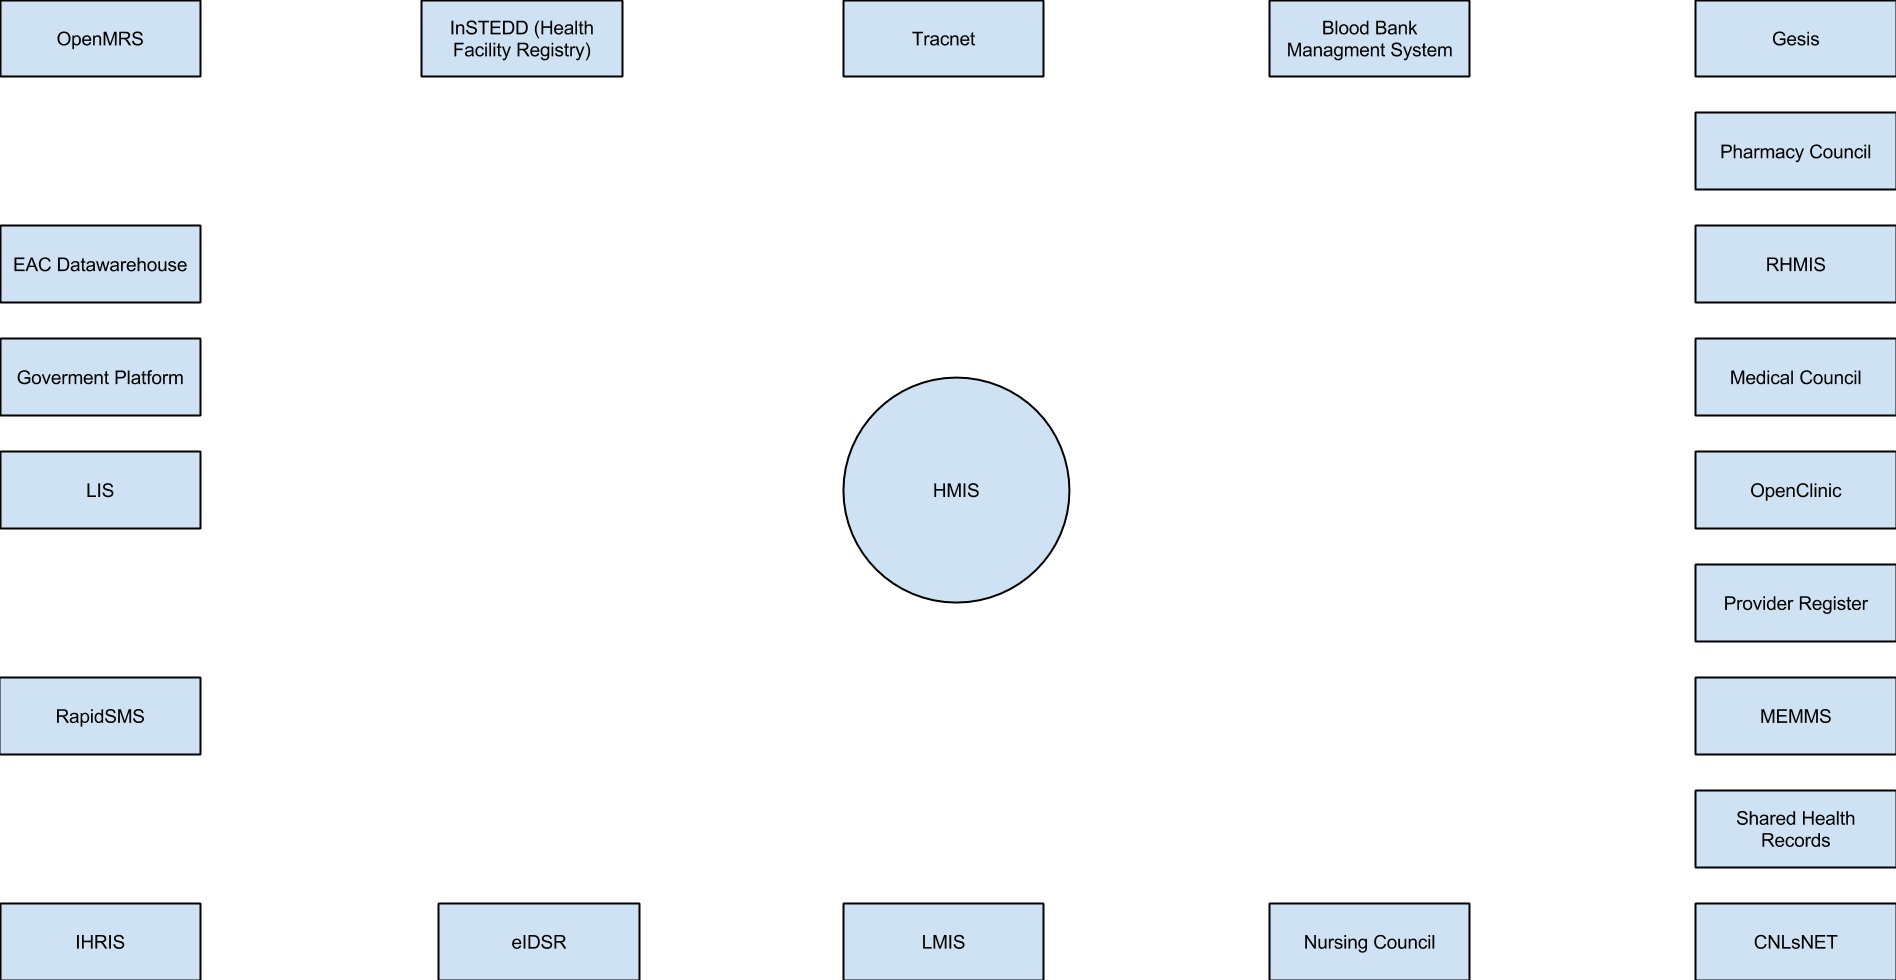
\includegraphics[width=12cm]{empirical/images/context.png}
\caption{Systems Currently in Use 2013}
\label{fig:systems_currently_in_use_2013}
\end{figure}
Besides the HMIS there are alot of systems that runs and has critical tasks that is not yet supported solely by DHIS2, see ~\ref{fig:systems_currently_in_use_2013}. These systems has varying tasks, but are all in some way related to HMIS.
Sharing data between these systems is crucial for maintaining an overview of the health status in all of Rwanda.
\subsection{DHIS2 enters Rwanda}




